% SPDX-License-Identifier: Apache-2.0
% Build from this directory with XeLaTeX, BibTeX, XeLaTeX, XeLaTeX.
% Source-authoring stage: compilation and final-page visual inspection belong to the package owner.
\documentclass[11pt,letterpaper]{article}
\usepackage[margin=.82in,headheight=16pt,footskip=28pt]{geometry}
\usepackage{fontspec}
\setmainfont{P052-Roman.otf}[Path=/usr/share/fonts/opentype/urw-base35/,BoldFont=P052-Bold.otf,ItalicFont=P052-Italic.otf,BoldItalicFont=P052-BoldItalic.otf]
\setsansfont{DejaVu Sans}[Scale=.87]
\setmonofont{DejaVu Sans Mono}[Scale=.76]
\usepackage{amsmath,amssymb,amsthm,mathtools}
\usepackage{microtype,graphicx,xcolor,booktabs,tabularx,longtable,array}
\usepackage{enumitem,fancyhdr,caption,needspace,titlesec}
\usepackage{tikz}
\usetikzlibrary{arrows.meta,positioning,calc}
\usepackage[numbers,sort&compress]{natbib}
\usepackage{xurl}
\usepackage[unicode,colorlinks=true]{hyperref}
\definecolor{ink}{HTML}{251B38}
\definecolor{purple}{HTML}{6541A5}
\definecolor{violet}{HTML}{916CC3}
\definecolor{pale}{HTML}{F2EDF8}
\definecolor{muted}{HTML}{62596D}
\definecolor{gold}{HTML}{A57A36}
\hypersetup{linkcolor=purple,citecolor=purple,urlcolor=purple,
 pdftitle={AUTONOMOUS ENTERPRISES: ACTIVATE. EVOLVE. SCALE. -- The Discoverability Compiler},
 pdfauthor={Vincent Boucher, MONTREAL.AI and QUEBEC.AI},
 pdfsubject={Finite decision-specific experiment construction, capability inheritance and honest enterprise evidence},
 pdfkeywords={discoverability, bounded errors, experiment design, capability construction, SUCCESSOR Omega}}
\urlstyle{same}
\setlength{\parindent}{1.1em}
\setlength{\parskip}{.24em}
\setlength{\emergencystretch}{2.5em}
\setlength{\tabcolsep}{4.5pt}
\renewcommand{\arraystretch}{1.17}
\widowpenalty=10000 \clubpenalty=10000 \displaywidowpenalty=10000
\setlist{leftmargin=1.5em,itemsep=.18em,topsep=.35em}
\captionsetup{font=small,labelfont=bf}
\titleformat{\section}{\large\bfseries\color{ink}}{\thesection}{.65em}{}
\titleformat{\subsection}{\normalsize\bfseries\color{ink}}{\thesubsection}{.65em}{}
\titlespacing*{\section}{0pt}{2.1ex plus .5ex minus .2ex}{.9ex}
\titlespacing*{\subsection}{0pt}{1.6ex plus .4ex minus .2ex}{.5ex}
\pagestyle{fancy}\fancyhf{}
\fancyhead[L]{\footnotesize\sffamily\color{muted} THE DISCOVERABILITY COMPILER}
\fancyhead[R]{\footnotesize\sffamily\color{purple} SUCCESSOR $\Omega$}
\fancyfoot[L]{\footnotesize\sffamily\color{muted} Boucher / MONTREAL.AI / QUEBEC.AI}
\fancyfoot[R]{\small\thepage}
\renewcommand{\headrulewidth}{.3pt}
\renewcommand{\topfraction}{.94}\renewcommand{\bottomfraction}{.85}
\renewcommand{\textfraction}{.07}\renewcommand{\floatpagefraction}{.8}
\newcolumntype{Y}{>{\raggedright\arraybackslash}X}
\newcolumntype{P}[1]{>{\raggedright\arraybackslash}p{#1}}
\newtheorem{theorem}{Theorem}[section]
\newtheorem{proposition}[theorem]{Proposition}
\newtheorem{corollary}[theorem]{Corollary}
\theoremstyle{definition}\newtheorem{definition}[theorem]{Definition}
\theoremstyle{remark}\newtheorem{remark}[theorem]{Remark}
\newcommand{\R}{\mathbb R}
\newcommand{\Z}{\mathbb Z}
\newcommand{\W}{\mathcal W}
\newcommand{\G}{\mathcal G}
\newcommand{\E}{\mathcal E}
\newcommand{\Pairs}{\mathcal P}
\newcommand{\supp}{\operatorname{supp}}
\newcommand{\status}[1]{\textsf{\small #1}}
\newcommand{\pending}{\textit{not yet recorded}}
\newcommand{\Om}{\texorpdfstring{SUCCESSOR $\Omega$}{SUCCESSOR Omega}}
\newcommand{\brand}{\texorpdfstring{TRANSFORMATIONAL META-AGENTIC $\alpha$-AGI}{TRANSFORMATIONAL META-AGENTIC alpha-AGI}}
\newcommand{\callout}[1]{\par\smallskip\noindent\colorbox{pale}{\begin{minipage}{\dimexpr\linewidth-2\fboxsep\relax}\vspace{.45em}\color{ink}#1\vspace{.45em}\end{minipage}}\par\smallskip}
\input{results-data.tex}

\begin{document}
\begin{titlepage}
\thispagestyle{empty}
\noindent{\sffamily\small\color{purple}MONTREAL.AI\quad / \quad QUEBEC.AI\quad / \quad RESEARCH EDITION}
\vspace{.65cm}

\noindent{\fontsize{30}{34}\selectfont\bfseries\color{ink}
AUTONOMOUS\\ENTERPRISES:\par}
\vspace{.25cm}
\noindent{\fontsize{24}{29}\selectfont\bfseries\color{purple}
ACTIVATE. EVOLVE. SCALE.\par}
\vspace{.55cm}
\noindent{\fontsize{22}{27}\selectfont\color{ink}The Discoverability Compiler\par}
\vspace{.25cm}
\noindent{\large Decision-separating measurements and scope-checked successors\par}
\vspace{.6cm}
\noindent{\sffamily SUCCESSOR $\Omega$ Harness\par}
\noindent{\small\sffamily\color{muted}Powered by TRANSFORMATIONAL INTELLIGENCE $\infty$\par}
\noindent{\small\sffamily\color{muted}and the applicable \$AGIALPHA utility\par}
\vspace{.65cm}
\noindent{\large Vincent Boucher\par}
\noindent{MONTREAL.AI and QUEBEC.AI\par}
\noindent{Montréal, Québec, Canada\par}
\vspace{.25cm}
\noindent{\small\color{muted}\PublicationDate\quad $\cdot$ \quad \RunIdentity\par}

\vspace{.65cm}
\noindent{\color{purple}\rule{\linewidth}{1.1pt}}
\vspace{.15cm}
\noindent{\small\bfseries Abstract}\par
\small
An enterprise can possess accurate readings yet lack an experiment that answers its customer's question. We construct a bounded software capability that turns permitted channels into decision-separating measurement programs. A finite integer-contrast grammar cancels declared additive nuisance; exact interval checks certify decisions under bounded error. The frozen compiler serves digital diagnosis, a synthetic mixture assay and a separately authored network successor. An independent reference agrees on 124 problems; conventional methods tie the development acquisition costs, and an adaptive control wins. Later verification covers 791 observation cells. A changed clock model invalidates inheritance; an authorized grammar expansion constructs a replacement. Across two retained 333-mission campaigns, reuse cuts counted construction work by 58.6\% at the 100-mission workload, but timing is unstable and centralized execution stays faster. The thin workbench adapter, executable interface and evidence docket preserve successful and rejected results. A separate 36-test local-EVM qualification exercises the existing Alpha contracts and adapter. The US\$100 $\rightarrow$ US\$10,000 commercial challenge is unproven: no executable offer or customer receipt exists, and complete cost is unknown. Native commissioning of this family, institutional admission and physical validation remain unestablished.
\normalsize
\vfill
\noindent\begin{minipage}{\linewidth}
{\footnotesize\sffamily\color{purple}EXECUTED SYNTHETIC SOFTWARE\quad $\cdot$ \quad EXPLICIT REFUSALS\quad $\cdot$ \quad REUSABLE CAPABILITY\par}
\smallskip
{\footnotesize\color{muted}Acquisition units are declared task costs. They are neither US dollars nor customer revenue.\par}
\end{minipage}
\end{titlepage}

\section{Build an experiment before demanding an answer}
In the held-out network model, an operator must choose a route while every raw measurement mixes path delay with an unknown clock offset and drift. A precise reading can still leave the required decision ambiguous. Repeating an uninformative observation does not create the missing distinction. The first useful product is therefore a measurement program: a permitted combination of readings that removes the modeled nuisance and preserves the answer the operator needs.

The constructive question is therefore: \emph{what measurement program would make the authorized decision possible?} The output sought here is an executable means of answering subsequent questions. It contains permitted channel acquisitions, a nuisance-canceling transformation, a robust decision certificate, a decoder and a scope that can be checked again when a successor changes the requirement.

This is a deliberately finite research result. Human and AI-assisted engineering specified the model class, grammar, implementation, tests and experimental protocol. The software then executes bounded construction and acquisition. It does not discover physical laws, invent arbitrary sensors or create its own customers. Those distinctions are central to the enterprise claim: useful software may precede a validated market, but the two must not be reported as the same achievement.

\callout{\textbf{The first product is an experiment the next mission can reuse.} Figure~\ref{fig:transformation} follows the retained network case from an ambiguous raw level to a checked route decision and a changed repair requirement. Its successor inherits valid construction structure, while the required answer is checked again.}

\input{figures/transformation.tex}

\subsection{An additive contribution inside an existing project}
The inherited system already contains experiment construction, representation compilers, robust completion, reusable execution boundaries and capability lineage. The foundation papers explicitly distinguish a changed formulation from improved search within one \citep{ti,learn,think,design,strategise,execute,evolve,economy}. Their executable companions are substantive prior work. In particular, \emph{Out-Learn} already synthesizes drift-rejecting measurement protocols and calibration; \emph{Out-Think} compiles purpose-preserving representations; \emph{Out-Strategise} constructs actions that tolerate unresolved uncertainty; and \emph{Out-Execute} preserves usable completion boundaries through change. This paper does not claim to originate those ideas.

The refreshed Alpha main source also includes a separate computational foundry of exact rational Walsh transforms, XOR convolution and inverse operators, together with capital and retention studies. Its independent joint planner ties the selected shared architecture, and a supplied specialist improves the particular inverse operation count. Those results and their excluded costs remain part of the comparison \citep{existingfoundry}. Our finite measurement compiler is an additional domain-specific capability at the existing workbench seam, rather than a replacement for that foundry or its review history.

\begin{table}[htbp]
\centering\small
\caption{Novelty statement and explicit boundary of the contribution.}
\label{tab:novelty}
\begin{tabularx}{\linewidth}{@{}P{.22\linewidth}Y@{}}
\toprule
Item & Concrete statement \\
\midrule
Inherited capability & Finite construction, exact references, source-bound artifacts, the Alpha workbench interface, existing lineage/recovery facilities and separate commissioning backends. \\
Restrictive assumption & The supplied observation interface must be accepted even when it cannot distinguish the beneficiary's required decisions. \\
New implementation & A bounded integer-contrast grammar compiled into a decision-pair cover, exact rational observation handling and scope-checked structural inheritance across three mission families. \\
New feasible activity & Within the admitted models, an operator can request a diagnostic decision, an assay disposition or a route/repair decision and receive a checked acquisition program or a complete scoped refusal. \\
Decisive experiment & Freeze the compiler, reveal a different inverse domain, retain only valid structure, reject a changed nuisance scope and reconstruct the missing capability without altering the original compiler or reference. \\
Not rebuilt & The native harness, wallet/admission system, shared runtime registry, contracts, release publisher, thermal instrument or existing six-stage Discovery Lab. \\
\bottomrule
\end{tabularx}
\end{table}

\subsection{The preceding failure changes the acceptance target}
The thermal Foundry research edition demonstrates a constructive progression from fixtures to a station, an instrument and a successor. Its retained metrology challenge also records a failure that the runtime did not detect: the predicted-versus-observed heat discrepancy was \(4.947712\%\), below its unchanged \(5\%\) rule, while an independently implemented reference found \(8.696402\%\) error relative to the model's true heat. Conventional engineering needed 384 initial readings against 672 for the proposed construction. The modeled centralized laboratory cost CAD~11,704.13 against CAD~12,164.13 for the shared arrangement \citep{thermalfoundry}.

These are simulated physics and conditional economics, not physical calorimetry or observed customer demand. Their lesson is operational: agreement with a convenient observable can be insufficient for the useful objective. Here, the acceptance obligation names \emph{every pair of modeled worlds that requires different decisions}. A good fit alone cannot discharge that obligation. The protection still depends on the correctness and completeness of the supplied world, nuisance and error models; no internal certificate can prove those assumptions from itself.

\section{Three candidate families and the choice of a flagship}
We developed three candidate families before selecting the implementation. Each would construct a reusable means of production, but each faces a different cheapest test.

\begin{longtable}{@{}P{.20\linewidth}P{.36\linewidth}P{.38\linewidth}@{}}
\caption{Candidates, downstream opportunities and early falsification.}\label{tab:candidates}\\
\toprule
Family & Bottleneck, construction and first deliverable & Downstream opportunities and cheapest falsification \\
\midrule
\endfirsthead
\toprule Family & Bottleneck, construction and first deliverable & Downstream opportunities and cheapest falsification \\\midrule
\endhead
Discoverability compiler &
An inherited interface can leave the required decision ambiguous. Synthesize nuisance-rejecting measurements and a finite robust decision program from already authorized channels. Existing exact arithmetic, finite search and workbench extension facilities suffice for a first software diagnostic protocol. &
Digital fault isolation; synthetic assay disposition; network route or repair diagnosis. Freeze the compiler, expose it to a new domain, and compare its complete result with an independently implemented optimizer using the same grammar. A mismatch, false refusal or unjustified acceptance falsifies the corresponding claim. \\[.35em]
Robust productive systems &
Expensive diagnosis may be unnecessary if a modular design works across the uncertainty class. Construct verified tolerance and reusable production boundaries. A first deliverable is a finite robust service configuration with an independently checked completion. &
Resilient software deployment; uncertain supply configuration; repairable process modules. Compare against a competent centralized robust optimizer on identical uncertainty and quality constraints. Much of this mechanism is already addressed by Out-Strategise and Out-Execute, reducing the additive scope here. \\[.35em]
Capability and commitment composition &
Several useful outputs may remain individually uneconomic because they each bear a shared setup cost. Combine existing capabilities with voluntarily accepted, conditional commitments. The first useful artifact is an auditable feasibility and funding schedule. &
Shared test access; coordinated software migration; pooled nonexclusive research services. Insert executable independent offers and cash timing, then check whether the package is still financeable. No such external offer is available in this record; Invent the Economy and Foundry already supply substantial modeled precedents. \\
\bottomrule
\end{longtable}

Discoverability was selected because a complete, inexpensive falsification is available before inventing demand or constructing physical equipment. The finite model gives an inspectable distinction between ambiguity, insufficient acquisition budget and unfinished search. The cross-domain successor can test whether the retained object is a reusable construction method rather than another rendering of one thermal output. This choice does not establish a new general algorithmic field: experimental design, bounded-error identification and set covering are established foundations \citep{pukelsheim,walter,chvatal}.

\section{A finite compiler of decision-relevant measurements}
\label{sec:model}
\subsection{Worlds, decisions, nuisance and acquisition}
A mission supplies a finite world set \(\W\), a required decision \(g:\W\to\mathcal D\), and \(n\) permitted channels. Channel \(i\) has known modeled response \(s_i(w)\), positive acquisition cost \(c_i\), and error radius \(\eta_i\geq0\). The integer matrix \(N\in\Z^{n\times m}\) describes the shared additive nuisance. One experiment acquires its selected channels according to
\begin{equation}
 y_i=s_i(w)+N_{i,:}\theta+\epsilon_i,
 \qquad \theta\in\R^m,\qquad |\epsilon_i|\leq\eta_i .
 \label{eq:observation}
\end{equation}
The same \(\theta\) applies within that experiment; its value may change between experiments. Every error vector in the declared box is admissible, and each experiment receives fresh errors. Here \emph{independent} describes a Cartesian feasible set, not an assumed probability distribution or a claim about stochastic independence in a laboratory.

A contrast is an integer vector \(a\in\Z^n\). It produces the observable
\begin{equation}
 z_a=a^\top y=a^\top s(w)+a^\top\epsilon
 \quad\text{when}\quad a^\top N=0 .
 \label{eq:contrast}
\end{equation}
The compiler's finite grammar \(\G\) restricts support size, coefficient magnitude and the \(\ell_1\) norm. It retains primitive vectors, \(\gcd(a_1,\ldots,a_n)=1\), with first nonzero coefficient positive. These conventions remove proportional sign copies; they do not enumerate all imaginable measurements. A contrast costs
\begin{equation}
 C(a)=\sum_{i:a_i\ne0}c_i,\qquad
 \rho_a=\sum_i|a_i|\eta_i,\qquad
 I_a(w)=[a^\top s(w)-\rho_a,\ a^\top s(w)+\rho_a].
 \label{eq:interval}
\end{equation}
Each nonzero-weight channel is read and charged once per experiment. Repeating a channel in a different contrast incurs a fresh acquisition and another charge. Reusing one raw reading across several contrasts changes the feasible transcript geometry and is outside this contract.

The relevant unknown is the decision, not necessarily the complete world. Define
\[
 \Pairs=\{\{u,v\}\subseteq\W:g(u)\ne g(v)\}.
\]
Worlds requiring the same action may remain indistinguishable. This purpose-specific quotient can reduce the obligation without weakening the externally specified task.

\subsection{A complete separation criterion}
\begin{theorem}[Robust decision separation under fresh bounded errors]
\label{thm:separation}
Let \(\E\subseteq\G\) be a static finite set of nuisance-canceling experiments, executed according to Equations~\eqref{eq:observation}--\eqref{eq:interval}. A decoder can return the correct decision for every modeled world and every admissible transcript if and only if
\begin{equation}
 \forall\{u,v\}\in\Pairs,\quad
 \exists a\in\E:\quad
 |a^\top(s(u)-s(v))|>2\rho_a .
 \label{eq:separation}
\end{equation}
\end{theorem}
\begin{proof}
The image of the channel-error box under \(a^\top\epsilon\) is exactly the interval \([-\rho_a,\rho_a]\). Consequently, the feasible transcript set for world \(w\) is the Cartesian product
\[
 T_{\E}(w)=\prod_{a\in\E} I_a(w).
\]
Fresh errors make every coordinate-wise choice attainable. Two such products intersect if and only if their intervals intersect in every coordinate. They are disjoint if and only if some experiment satisfies the strict inequality in Equation~\eqref{eq:separation}.

If all different-decision world pairs have disjoint transcript sets, every feasible transcript is compatible only with worlds sharing one decision. Returning that decision is correct. Conversely, if a different-decision pair overlaps in every coordinate, choose one point from each interval intersection. The resulting identical transcript is feasible in both worlds. Any decoder must return the same answer on it and therefore fails in at least one of them. A refusal to decide does not count as a correct completed decision.
\end{proof}

Touching intervals overlap at their endpoint. Replacing \(>\) by \(\geq\) would incorrectly certify such a boundary. The implementation's negative witness takes the midpoint of each pairwise intersection. Twice this midpoint is an integer because centers and radii are integers; it is therefore representable without rounding. The witness proves ambiguity inside the complete admitted grammar, not impossibility for a better sensor, a different error model or an expanded grammar.

\begin{corollary}[Exact finite cover formulation]
\label{cor:cover}
For each \(a\in\G\), let \(S_a\subseteq\Pairs\) contain the pairs separated by that contrast. Minimum additive acquisition cost among static grammar programs is
\begin{align}
 \min_{x_a\in\{0,1\}} \quad & \sum_{a\in\G} C(a)x_a \label{eq:cover}\\
 \text{subject to}\quad&
 \sum_{a:\,p\in S_a}x_a\geq1 \qquad(p\in\Pairs). \nonumber
\end{align}
If some \(p\) belongs to no \(S_a\), the complete grammar cannot identify the decision.
\end{corollary}
\begin{proof}
The constraints are exactly Theorem~\ref{thm:separation}, and the objective is the stated fresh-acquisition cost. Repeating an identical experiment does not enlarge worst-case pair separation under independently chosen bounded errors, so a static set suffices.
\end{proof}

This is a reduction to an established optimization problem, not a claim to have invented set cover. The implementation first enumerates the admitted contrasts, collapses equal coverage to a cheapest representative and removes a contrast whose coverage is contained in another no-more-expensive one. A greedy feasible cover supplies an incumbent. Exhaustive branch-and-bound then selects an uncovered pair and explores its covering candidates, memoizing the cheapest cost for each covered-pair state. Every feasible improvement must take a candidate covering the selected pair; positive costs and the incumbent justify the pruning. A completed search therefore establishes the minimum \emph{within this static grammar}. An adaptive decision tree can have a lower worst-case cost, as our control experiment demonstrates.

\subsection{A small constructive example}
Consider three equally priced readings at \(t=0,1,2\), with unknown offset and drift,
\[
 N=\begin{pmatrix}1&0\\1&1\\1&2\end{pmatrix},
 \qquad a=(1,-2,1)^\top.
\]
Then \(a^\top N=0\). With channel-error radius one, \(\rho_a=4\). Let the two modeled signals be \(s(u)=(0,0,0)\) and \(s(v)=(0,6,0)\), requiring different actions. Their contrast centers are \(0\) and \(-12\); the intervals \([-4,4]\) and \([-16,-8]\) are disjoint. Three acquired readings yield a robust decision despite unrestricted affine nuisance.

A single channel cannot cancel the offset; two distinct times cannot cancel both nuisance columns with a nonzero contrast. Under this illustrative grammar, constructing the three-reading interface creates an available decision. This algebraic example explains the mechanism; it is not an additional empirical result or a model of a commissioned physical sensor.

\begin{figure}[htbp]
\centering
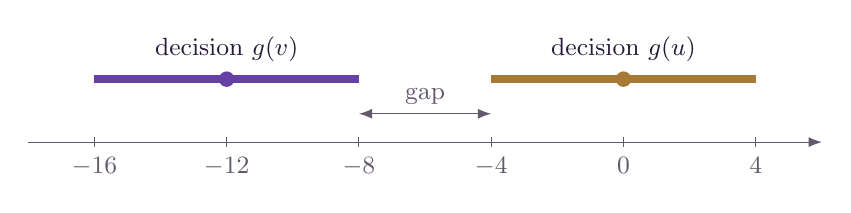
\begin{tikzpicture}[x=.42cm,y=.8cm,font=\small,>=Latex]
 \draw[->,draw=muted] (-18,0)--(6,0);
 \foreach \x in {-16,-12,-8,-4,0,4}{
   \draw[draw=muted] (\x,.08)--(\x,-.08);
   \node[below,text=muted] at (\x,-.08) {\(\x\)};
 }
 \draw[line width=3pt,draw=purple] (-16,1)--(-8,1);
 \fill[purple] (-12,1) circle (2.8pt);
 \node[above,text=ink] at (-12,1.12) {decision \(g(v)\)};
 \draw[line width=3pt,draw=gold] (-4,1)--(4,1);
 \fill[gold] (0,1) circle (2.8pt);
 \node[above,text=ink] at (0,1.12) {decision \(g(u)\)};
 \draw[<->,draw=muted] (-8,.45)--(-4,.45);
 \node[above,text=muted] at (-6,.45) {gap};
\end{tikzpicture}
\caption{The illustrative contrast cancels offset and drift. Correctness concerns the entire modeled intervals, including their endpoints. An apparently central or likely observation cannot substitute for separation of those intervals.}
\label{fig:interval}
\end{figure}

\section{Executable capability, scope and succession}
\label{sec:implementation}
The frozen core has no third-party runtime dependencies and exports \texttt{createCompiler}, \texttt{validateProblem}, \texttt{inspectProgram} and \texttt{executeProgram}. It is bounded to ten channels, 64 worlds and four nuisance columns; coefficient magnitudes are at most three and total absolute weight at most twelve. Construction retains at most 1,024 templates, emits at most 128 selected experiments and limits serialized results. Input framing rejects non-JSON objects, accessors, sparse arrays, forbidden keys, invalid Unicode and non-safe integer fields \citep{compiler}.

The compiler distinguishes four operationally important outcomes. \status{COMPILED} includes a separating optimum within the mission acquisition budget. \status{OVER\_MISSION\_BUDGET} retains an identified optimum that exceeds that budget. \status{UNIDENTIFIABLE\_WITHIN\_GRAMMAR} requires complete template construction and an uncovered different-decision pair. \status{BUDGET\_EXHAUSTED} means search, framing, retention or serialization did not complete; it cannot be used as a negative scientific result. The logical work meter and cooperative checkpoints are separate from wall-clock execution deadlines.

A program binds the complete canonical problem, including world responses, decisions, channel costs, nuisance, grammar and budget. Before decoding, \texttt{inspectProgram} recomputes legality, nuisance cancellation, response intervals, cost and pair separation. It does not independently redo the minimum-cost optimization; independent references address that claim. Observations are either safe integers or exact numerator/positive-denominator pairs. \texttt{executeProgram} uses \texttt{BigInt} cross-multiplication to compare them with interval bounds. It returns \status{DECIDED}, \status{OUT\_OF\_SCOPE} or \status{AMBIGUOUS}; hidden synthetic truth belongs only to the evaluator.

This exact transport was a substantive repair. Early review identified that the declared continuous observation model did not fit an integer-only decoder, and also found a coerced Boolean identity. The frozen source has rational observation handling and strict identity regressions. Correcting these defects is recorded engineering, not autonomous self-repair by the enterprise.

\subsection{What survives a changed mission}
The reusable library stores immutable legal contrast templates, keyed by schema, channels, nuisance and grammar. It does \emph{not} cache the answer, world responses, goal-pair cover or acceptance. Those are recomputed for each mission. A change in required decisions can therefore reuse the same structural search while constructing a different program. A changed nuisance matrix or grammar forces a new library key. A previously emitted program fails direct scope inspection on any changed problem.

The cache is bounded to eight entries and is in-process. Restart discards it; durable journal recovery is a separate runtime concern. This distinction prevents a memory optimization from being presented as an independently owned, persistent enterprise capability. The source-bound program, evidence and lineage proposal are the objects that a maintained harness can review and retain.

\begin{table}[htbp]
\centering\small
\caption{Causal roles of the six Out-stages and executed ablations. These measurements were made in portable V8; their logical work units are separate from the direct Node test results.}
\label{tab:ablations}
\begin{tabularx}{\linewidth}{@{}P{.17\linewidth}P{.34\linewidth}Y@{}}
\toprule
Stage & Constructive role & Removal or change and observed consequence \\
\midrule
Out-Learn & Construct informative permitted measurements. & Primitive-only support one yields zero legal templates and a complete within-grammar refusal. \\
Out-Think & Preserve the required decision while removing irrelevant distinctions. & Digital health needs 5 goal pairs instead of repair's 15; work is 2,355 versus 2,506, with acquisition cost 6 in both. \\
Out-Design & Synthesize a realizable nuisance-canceling program. & Removing magnitude-two coefficients from the tested three-support grammar leaves zero legal templates and refusal. \\
Out-Strategise & Resolve decision-relevant uncertainty and neutralize declared drift. & Omitting drift proposes cost 5, but the original scope gate rejects it. Six tested true-drift acquisitions under that wrong model return out-of-scope. \\
Out-Execute & Reuse a valid structural boundary and reconstruct current responses. & Cold compilation costs 2,506 logical units; reused structure costs 731, with identical program and acquisition cost 6. Restart requires rebuilding. \\
Out-Evolve & Test a changed requirement without silently widening the parent's claim. & Post-freeze route choice costs \HoldoutRouteCost; finer repair costs \HoldoutRepairCost. Changed quadratic drift invalidates the old grammar; explicit reconstruction costs \HoldoutRebuiltCost. \\
\bottomrule
\end{tabularx}
\end{table}

The wrong-clock test is a useful negative control, not a general detector of every model error. Some incorrect models can generate observations inside the accepted intervals and still produce a wrong real-world decision. The conditional theorem cannot settle that problem. Field calibration, independent measurement and model revision remain necessary before physical use.

The accepted cache behavior reduces 1,775 metered operations in the stated repeat case. It does not reduce that case's acquisition cost and does not establish cheaper full production once engineering, checking, inference and support are charged. A changed grammar producing a cheaper answer on a changed scope is a new qualification, not a clean improvement comparison against the old task. Neither result is general recursive self-improvement.

\Needspace{5\baselineskip}
\section{Experiments: useful construction, conventional ties and a held-out successor}
\label{sec:experiments}
\subsection{Freeze, independent reference and decision accuracy}
The compiler was frozen at Alpha commit \texttt{\CoreShortRevision}; its complete SHA-256 identity appears in Appendix~\ref{sec:identities}. The independent reference has a separate source hash. It was authored separately within the same research effort, which provides implementation diversity but not institutional independence or an external audit. The post-freeze family was constructed after the compiler freeze; its exact source and ordering are retained in same-team run records, rather than an external preregistration \citep{compiler,run}.

The direct core suite records \CoreTests{} passing tests on Node \ObservedNodeVersion. The workbench adapter and delivery suites add \AdapterTests{} and \DeliveryTests{} checks, respectively: \TotalNodeTests{} direct Node checks with no failures or skips. These are observations on that actual runtime. They are not qualification on the repository's pinned Node 22.17.1, an installed four-repository release or an EVM execution.

The independent numerical comparison covers \ReferenceCases{} complete static checks: four development tasks and 120 generated finite problems. The generated cases include 50 compiled programs, 66 complete within-grammar refusals and four optima above the mission acquisition budget. Ten additional adversarial controls exercise declared boundaries. Agreement means agreement for these explicit finite cases, not an error-rate estimate for a population of real diagnostic problems. A later exhaustive observation-cell check has status \ObservationCellStatus{} and count \ObservationCellCount{}. It partitions each selected experiment axis at every independently recomputed interval endpoint, tests endpoints, open regions and exterior cells using exact rational representatives, and enumerates the Cartesian products. Across the three compiled held-out programs, 147 cells return the required decision and 644 return out-of-scope, with zero mismatches or ambiguous acceptances. Three stale-parent-scope controls also reject. This is later verification of the retained family, not pre-evaluation preregistration.

\subsection{Three materially different mission families}
The first family diagnoses a digital module. Its response signatures come from executable XOR, AND, OR, NAND and stuck-output functions under four input stimuli, with reference channels and affine nuisance. One requirement asks for a health decision; another distinguishes the repair-relevant function. Both yield cost six using two contrasts. The second family uses a two-component, four-band synthetic mixture model with blank channels. Concentrations are drawn from a bounded finite catalogue; disposition and exact-quantity requirements yield cost seven using one contrast. Every synthetic acquisition is freshly executed, and its truth is withheld from the decoder.

The third family is independently authored network tomography revealed after the freeze. It changes the inverse domain and then changes the requirement within it. Route choice needs cost \HoldoutRouteCost{} and uses a library with \HoldoutRouteTemplates{} legal templates. Exact edge-and-severity repair needs cost \HoldoutRepairCost{} and reuses that structural library while recalculating the decision obligations. Quadratic clock drift invalidates the old grammar: complete construction yields \HoldoutInvalidTemplates{} legal templates and a refusal. An explicitly expanded grammar with support at most four, coefficient magnitude at most three and \(\ell_1\) limit eight constructs a new program costing \HoldoutRebuiltCost{} from \HoldoutRebuiltTemplates{} legal templates.

\begin{table}[htbp]
\centering\small
\caption{Acquisition results. All numbers are declared weighted acquisition units. Conventional static and adaptive references receive the same permitted measurement grammar. A dash denotes a complete refusal, not a zero-cost successful mission.}
\label{tab:results}
\begin{tabularx}{\linewidth}{@{}Yrrrr@{}}
\toprule
Mission requirement & Compiler & Static & Adaptive & Templates \\
\midrule
Digital repair & 6 & 6 & 6 & 6 \\
Digital health & 6 & 6 & 6 & 6 \\
Mixture disposition & 7 & 7 & 7 & 6 \\
Mixture quantification & 7 & 7 & 7 & 6 \\
Held-out route choice & \HoldoutRouteCost & \HoldoutRouteCost & \HoldoutRouteCost & \HoldoutRouteTemplates \\
Held-out exact repair & \HoldoutRepairCost & \HoldoutRepairCost & \HoldoutRepairCost & \HoldoutRouteTemplates \\
Changed quadratic drift, old grammar & --- & --- & --- & \HoldoutInvalidTemplates \\
Changed quadratic drift, enlarged grammar & \HoldoutRebuiltCost & \HoldoutRebuiltCost & \HoldoutRebuiltCost & \HoldoutRebuiltTemplates \\
Separate adaptive-advantage control & 3 & 3 & 2 & \AdaptiveControlTemplates \\
\bottomrule
\end{tabularx}
\end{table}

The quadratic successor is not a pure six-to-four improvement. Both its nuisance scope and admitted construction grammar change. Its value is evidential: the system refuses an invalid inheritance, constructs new permitted structure and requalifies the changed task. The frozen compiler and the independent reference remain unmodified. The conventional methods tie every listed development and held-out acquisition result; the adaptive control wins two versus three. These are evidence against a blanket superiority claim and useful checks that the benchmark does not require the proposed method to win.

The three families share a finite inverse-problem interface but differ in what generates their signals and what decisions they support. That is more than three copies of a stored output, yet it remains narrower than arbitrary scientific discovery. The signal model, finite catalogue and lawful permission to acquire each channel are supplied. Real uncertainty outside those declarations is not covered.

\subsection{Inheritance, rejection and the cost of improvement}
A non-inheriting compiler reconstructs the same legal contrasts before each mission. A cached compiler retains their immutable structural library. The repeated digital-repair ablation gives identical programs and acquisition cost, with logical work declining from 2,506 to 731. Its purpose is to demonstrate what was inherited: complete enumeration of a structure whose key is unchanged. It does not treat previous construction as free; the cold construction remains part of the lineage cost.

The scope-changing successor and malformed-certificate tests retain rejected attempts. They distinguish a useful acceptance from a convenient edited criterion. The theorem's decision requirement, error bounds and exact comparison are not weakened to rescue a failing program. A changed problem is named and qualifies separately. Promotion into a native capability inventory still requires the existing owner's acceptance path; the research compiler cannot authorize its own operational authority.

A complete improvement account must charge proposal generation, sandbox execution, reference evaluation, qualification, failure and monitoring, then compare under the original acceptance test. The present arithmetic/work and wrapper records cover only their declared portions. Human engineering and full monetary overhead remain unknown. The accepted structural optimization and rejected invalid scopes are concrete software results; a self-directed general improvement system is not established.

\subsection{Load, contention and recovery}
Repeated compilation can measure execution capacity without measuring customer demand. The load protocol therefore retains mission composition, concurrency, source/runtime identity, quality, errors, wall time, p50/p95 latency, work and human intervention separately. Identical cached requests alone would understate heterogeneous construction and contention. Fresh, cached and centralized reference treatments require the same decision target.

\begin{table}[htbp]
\centering\small
\caption{Actual inherited-workbench load measurements. All world decisions were sampled and independently checked against the declared models. Service latencies exclude pending queue wait and are milliseconds; concurrency counts cooperative calls in one Node process.}
\label{tab:scale}
\begin{tabularx}{\linewidth}{@{}rYrrrr@{}}
\toprule
Missions & Composition / concurrency & Completed & Errors & p50 & p95 \\
\midrule
1 & \ScaleOneComposition & \ScaleOneCompleted & \ScaleOneErrors & \ScaleOnePFifty & \ScaleOnePNinetyFive \\
10 & \ScaleTenComposition & \ScaleTenCompleted & \ScaleTenErrors & \ScaleTenPFifty & \ScaleTenPNinetyFive \\
100 & \ScaleHundredComposition & \ScaleHundredCompleted & \ScaleHundredErrors & \ScaleHundredPFifty & \ScaleHundredPNinetyFive \\
\bottomrule
\end{tabularx}
\end{table}

\ScaleNarrative{}

\begin{figure}[htbp]
\centering
\includegraphics[width=\linewidth]{figures/load-results.png}
\caption{Two retained single-host campaigns at 100 heterogeneous missions. Structural reuse reduces counted compiler work in both. The workbench timing ordering reverses; direct centralized execution remains faster. The direct solver meets the same scientific quality target but omits workbench artifacts. All paths use the same acquisition units. These two campaigns provide no controlled causal allocation of timing overhead, confidence interval or general latency claim.}
\label{fig:load}
\end{figure}
No synthetic throughput observation establishes independent validator capacity, financially realizable order volume or 100 viable businesses. Outages, malformed inputs, duplicate requests, exhausted budgets and restart uncertainty belong in the failure account. A replay of a retained receipt demonstrates that receipt's inspection path; only a new execution can supply new operational evidence.

\subsection{Post-freeze review: preserve the experiment, correct the implementation}
The numerical campaigns above use the retained \texttt{1.0.0-experimental} compiler. A subsequent public review found that a mission whose worlds all require the same decision still enumerated the measurement grammar before selecting the empty program. Under a 2,000-unit work budget, the same-goal digital control exhausted its resources despite needing no acquisitions. The separately identified \texttt{1.0.1-experimental} correction returns the checked zero-experiment program after framing, preserving metering and serialization bounds. It completes that control in 248 counted work units at zero acquisition cost. This is an ordinary review-assisted correction, not autonomous invention or general recursive self-improvement.

The corrected source passes 22 core checks, including the new regression, plus the unchanged 13 adapter and seven delivery checks on Node 24.19.0. A separate comparison re-executes 128 already-public inputs: 124 reference cases and four former held-out cases. All 111 nontrivial results from fresh compiler instances match the frozen implementation after removing only the version field; the 17 same-goal cases retain their programs while avoiding construction. The shortcut does not warm the grammar cache for a mission that already knows its decision. The independent checker accepts all 61 returned programs. These are post-review regressions, not a second blinded successor study or a replacement for the original timing measurements. Exact frozen compiler/test bytes and the original browser bundle are preserved; the current interface embeds the corrected compiler. The amendment, commands and raw checks are in \path{evidence/post-review/}.

\section{One enterprise journey inside the existing architecture}
\label{sec:architecture}
The product identity is \brand. The intended journey follows
\emph{Identify; Out-Learn; Out-Think; Out-Design; Out-Strategise; Out-Execute; Out-Evolve}.
Table~\ref{tab:ablations} gives these stages causal roles. A screen bearing their names is not their implementation.

The smallest working research journey accepts a bounded mission, compiles a measurement program, executes a synthetic acquisition, decodes the observations, checks the evidence and exposes a successor proposal. Its thin extension uses the maintained \texttt{createWorkbench(adapters)} seam; it does not supply a fifth platform. \AdapterImplementationNarrative{} The public experience must state whether a result is a newly executed synthetic run, a retained replay or an unavailable backend operation. Wallet-free inspection does not imply contract settlement.

The architecture docket records exact source paths, interfaces, tests and ownership boundaries for each required component. The abbreviated map below distinguishes reusable existing implementations from this candidate's remaining integration. Repository-local tests are named evidence locations; their existence does not mean they were rerun in this experiment \citep{alpharuntime,alphasuite,jobs,manager,fleet,coordination}.

\begin{longtable}{@{}P{.15\linewidth}P{.39\linewidth}P{.40\linewidth}@{}}
\caption{A--H architecture map. Existing owners retain their components; the candidate owns only its additive compiler, narrow adapter and research material.}\label{tab:architecture}\\
\toprule
Component & Actual source and interface & Tests, owner boundary and candidate gap \\
\midrule
\endfirsthead
\toprule Component & Actual source and interface & Tests, owner boundary and candidate gap \\\midrule
\endhead
A. Insight &
Alpha's \texttt{discovery.py} consumes inspectable supplied excerpts, interval scores and an exact allocation model to draft opportunities and plans. &
\texttt{test\_insight\_discovery.py}; Alpha Insight owner. Supplied sources are not autonomously authenticated market foresight. Candidate finite models and decisions are authored inputs; a full source-to-FusionPlan discovery service is not established here. \\[.3em]
B. Nova-Seeds &
\texttt{NovaSeed.sol} seals capsule/plan/evidence hashes, job count, metadata and parent in an ERC-721 genome. Studio and \texttt{ascension.py} handle the off-chain handoff. &
Native handoff and lifecycle contract tests; Ascension/Studio owner. No Discoverability-linked seed was minted. Hash commitments do not provide encryption recovery, data rights or legal ownership of a business. \\[.3em]
C. MARK / risk oracle &
\texttt{AscensionMark.sol} and \texttt{AscensionRiskOracle.sol} implement admitted funding, review, expiry, job routing and refunds. &
Lifecycle/settlement Solidity suites; Ascension owner. Historical source/configuration are audited below; this compiler run does not establish fresh chain readiness or funded operation. \\[.3em]
D. Sovereign / Business &
Alpha's successor workbench and journal contain mission, budget, authority, queue, obligations, stop and recovery paths. The enterprise facade is an existing owner's separate lane. &
Workbench/state/recovery tests; native harness owner. Candidate wrapper operation is bounded research execution. The name confers no legal sovereignty, unlimited authority or completed production enterprise. \\[.3em]
E. Marketplace &
The selected Alpha path has bonded offers and weighted selection. Jobs v0 exposes a separate JobRegistry lifecycle; Manager has an alternative USDC route. &
Market and successor-adapter contract tests; backend owners. Generic auction, universally cheapest execution and interchangeable settlement semantics are not claimed. No new candidate job is financially settled. \\[.3em]
F. Agents / Jobs &
Alpha's workbench runs bounded tool work; Fleet supplies qualified execution and internal review through its supervisor; Jobs supplies its actual commissioning path. &
Candidate core/adapter/delivery suites plus inherited runtime tests; Alpha/Jobs/Fleet owners. Deterministic workers are disclosed. This experiment does not demonstrate remote Fleet execution, unrestricted model agency or a completed four-repository round trip. \\[.3em]
G. Architect &
Compiler proposals, independent numerical comparisons, scope checks and existing candidate/state/mission lineage provide a controlled improvement path. &
Held-out and ablation evidence; candidate author plus native promotion owner. Current certificates and a changed-scope refusal operate. Institutional promotion, field monitoring and live rollback remain separate acceptance gates. \\[.3em]
H. Council / CLUB &
Actual Ascension admission, stake, conflicts, selected committees and vote thresholds; separate producer and acceptance addresses are enforced in source. &
Risk/market/settlement tests; contract admission authority. Address separation does not prove independent beneficial control. Compiler acceptance and internal Fleet review do not constitute an independent Validator Council approval. \\
\bottomrule
\end{longtable}

The native owner has agreed that reviewed adapters compose through the repository-owned \path{examples/successor-workbench/native.mjs} seam. The candidate supplies its pure wrapper; a focused registration remains a separate reviewed integration. The held harness/bridge reviews are not bypassed. The final source refresh observes main \texttt{e7fbd7e7}, incorporating the owner's PR4873 correction of the failed \texttt{8f13b39e} qualification. Main/release qualification remains with that owner; the maintained record still reports unresolved qualification and restriction scope.\par

The four repositories retain different responsibilities. Alpha organizes the mission and evidence. Jobs exposes its selected commissioning and AGIALPHA settlement system. Fleet supplies execution and the actual qualified review facilities. Manager supplies management and a distinct USDC settlement alternative. A source-compatible receipt is not evidence that all four installed releases have accepted it.

Coordination is through issue \#4850 and focused candidate PR \#4872. The original audit pinned Alpha \texttt{61532fb8}; subsequent source inspection refreshed Alpha main to \texttt{8f13b39e}, containing the merged \#4855 work. The compiler freeze remains its own identity. The held native harness \#4863 and stacked Ascension bridge \#4865 keep their owners and unresolved acceptance boundary. No held implementation is copied into this candidate to bypass review. Existing papers and research URLs remain intact \citep{coordination,compiler,existingfoundry}.

\section{Contract and settlement evidence: exact backend, exact limit}
\label{sec:contracts}
The contract audit begins with Alpha's \texttt{CURRENT\_MAINNET\_DEPLOYMENT} and its deployment manifest, rather than an old release claim. The five-contract suite is AscensionAccess, NovaSeed, AscensionRiskOracle, AscensionJobMarket and AscensionMark. Its published deployment identifies source \texttt{c0fc5217} and Ethereum block 26,220,072, observed on 18 October 2026 at 14:51:02.815 UTC. The audit compared the five contract files and their token helper with the inspected main source and found the same file bodies. That is source-file equality, not a new chain observation \citep{alphadeployment,alphasuite}.

The machine-readable \path{contract-manifest.json} records chain, addresses, source revision, published ABI and runtime bytecode hashes, configuration and observation time. Complete ABI bytes are not bundled in that docket, and fresh RPC verification was unavailable. Its runtime identities are historical deployment assertions, not freshly observed \texttt{eth\_getCode} results. The recorded readiness flags were false. The suite has no global pause; that fact does not authorize funding, establish admission or make every operation ready.

\subsection{Admission, seed commitments and reviewed funding}
Alpha's actual fixed ENS roots are \texttt{*.alpha.agi.eth} for Business, \texttt{*.alpha.agent.agi.eth} for Agent and \texttt{*.alpha.club.agi.eth} for Validator. A live matching ENS owner also needs unexpired governor admission; an NFT does not confer validator eligibility. Wrapped names must be live and owned by the admitted account. Canonical labels and expiry bounds are enforced in source. These are this suite's roots, not a rule that may be transplanted into Jobs or Manager.

NovaSeed's seal binds a capsule hash, plan root, evidence hash, 1--128 jobs, metadata URI and parent. Creating a child requires current parent ownership. The immutable genome records the creator; ERC-721 transfer changes token ownership. The contract does not encrypt a capsule, deliver a decryption secret, license external data or transfer the original campaign business's authority. Recovery depends on the actual off-chain sealing mechanism and the holder of its recovery material.

The risk oracle's published configuration has quorum two, maximum risk 2,000 basis points and a minimum stake of ten AGIALPHA. Rounds last seven days and bind the current seed owner. Reviewers exclude that owner and the seed creator; green status rechecks current eligibility and supporting reviewers. Availability has bounded capacity and time, and stake locks can outlast an individual reservation's early release. These conditions are operational source rules, not a compliance guarantee.

MARK supplies a finite lot-funding mechanism. For current supply \(s\), count \(q\), base \(b\) and slope \(d\), its integral quote is
\begin{equation}
 Q(s,q)=qb+d\,q\bigl(2s+q-\mathbf1_{\{q>0\}}\bigr)/2 .
 \label{eq:mark}
\end{equation}
This arithmetic sum is not a generic DEX price. Campaign opening binds an eligible owner and a green seed, a reachable target, a funding window no longer than 30 days and an execution window longer than three days but no longer than 90. Buying and blooming recheck the relevant admission, risk and owner state. During Funding, selling retains an exit path even when admission or risk has expired; it is not conditioned on the funding deadline in the same way as buying.

Blooming ends curve redemption. Routing requires an exact indexed plan proof, an unposted job index, adequate reserve and time for the auction, execution and review. MARK approves the exact bounty and resets the allowance. It is the escrow client. Terminal job refunds return to campaign reserve once. Closing and pro-rata reclamation follow their actual state and time conditions; floor division leaves the last claimant the remaining rounding dust. Lot ownership is not company equity or a guaranteed principal repayment.

\subsection{Marketplace selection and settlement conservation}
The Alpha marketplace bounds bounty, auction and execution windows, reserves bidder bonds and retains at most 32 one-per-agent offers. Its score combines normalized price and duration with a bounded reputation discount; ties resolve by price, duration and address. This is not a guarantee of the fastest or cheapest possible worker. Expired or newly ineligible bids can be excluded at award. If no eligible offer remains, the bounty is refunded and bonds unlock.

Delivery requires the assigned eligible worker, a nonzero evidence hash and bounded URI before the deadline. Three distinct validators are selected, excluding the business, escrow client and worker. Two approvals pay; two rejections slash. Eligibility is rechecked at the decision. A late worker can time out and be slashed, but a missing review quorum produces a full bounty refund and unlock without a reputation decrement or worker slash. Those failure modes must remain distinct.

For gross bid price \(p\) in token base units, each of the two paid approving validators receives gross allocation \(e\), and the worker gross allocation is \(w\):
\begin{align}
 e&=\left\lfloor\frac{\left\lfloor500p/10000\right\rfloor}{2}\right\rfloor
   =\lfloor p/40\rfloor,& w&=p-2e, \label{eq:alloc}\\
 B&=\lfloor w/100\rfloor+2\lfloor e/100\rfloor . \label{eq:burn}
\end{align}
Burning is rounded separately on those payouts. Thus \(p=100\) yields \(e=2\), \(w=96\), \(B=0\); \(p=104\) yields \(B=1\); and \(p=1000\) yields \(B=9\), rather than \(\lfloor p/100\rfloor=10\). Net worker and validator payouts, actual burned units and the unused bounty refund conserve escrow. A slashed bond separately burns \(\lfloor\text{bond}/100\rfloor\) and returns the remainder according to the failure path. Refunds are single-use. These are not claims that every AGIALPHA transfer burns one percent.

The supplementary arithmetic reference enumerated 9,901 prices from 100 through 10,000 and 441 lot-curve cases using exact \texttt{BigInt}. All declared arithmetic checks passed; the maximum gap between \(\lfloor p/100\rfloor\) and the payout-wise burn in that bounded enumeration was two base units. This checks formulas, not Solidity storage transitions, token balances, overflow reverts or adapter receipts.

\subsection{Two other settlement systems remain separate}
Jobs v0 has its own deployed contract set, pause state, ENS/role rules, stake and first-eligible application lifecycle. Its historical deployment record described managed components paused, a separate per-job collateral rule and commit/reveal validation. Alpha's lack of a global pause cannot be used to infer Jobs readiness. Historical receiver profiles likewise cannot silently become trust in newly selected addresses \citep{jobs}.

Manager's route uses USDC with six decimals and its own configurable admission and separate intake/settlement controls. It is an alternative explicitly priced route, not an automatic conversion or a second charge layered onto an Alpha AGIALPHA job. Alpha's canonical token has 18 decimals. Economic utility in either route is not a token-appreciation forecast \citep{manager}.

A genuine existing test path, \path{tests/contracts/test/ascension/successor-adapter.test.js}, executes the Solidity suite in an unforked local Hardhat EVM and exercises the Python journal/adapter. Authorized execution with the exact npm lock and hash-locked Python environment resolved missing dependencies and restricted child-process output without changing source, assertions or security settings. The interrupted first handoff retained receipts and compiler artifacts but lost its full test-console output and exit receipt. That limitation remains recorded; a later data-only reconciliation passed 106 checks.

To close the specific custody gap, a supplementary qualification on 23 October 2026 at 01:50:49 UTC executed the same 36 unchanged tests: 15 lifecycle/identity, 15 marketplace/failure/recovery/rounding, three settlement-conservation and three native-adapter cases. All passed with actual exit code zero in 12.354 seconds. Full stdout/stderr, command, timestamps and before/after hashes of 54 executable source, configuration and lock files are retained in \path{evidence/local-evm/qualification-02/}. The run reused pinned dependencies and compiler artifacts; it is not a fresh compilation. The adapter paid a correctly reported negative evaluation without admitting the candidate, preserved idempotent settlement import, rejected an artifact mismatch and refunded/unlocked after missing quorum. A separate disposable fixture records all five deployed runtime identities and configuration; it does not retroactively fill missing observations in the first receipts. These tests establish existing adapter behavior at Alpha source \texttt{61532fb8}, not Discoverability commissioning or an installed four-repository journey. All balances and actors are deterministic local fixtures. No mainnet transaction, external financial signing or transfer was performed.

Later review found that the historical custody wrapper could record a failed subprocess while returning process status zero. Its successful test and fixture receipts both record actual exit zero and remain unchanged. A new \texttt{qualification-runner.py} preserves evidence before propagating failure or timeout. Seven deterministic operating-system subprocess controls pass, covering success, test and fixture failures/timeouts, nonempty-output refusal and command-line refusal. These controls qualify failure reporting for future use; they are not another Solidity execution. The executed historical wrapper remains preserved with its original evidence.

\section{Commercial value and autonomy remain separate hypotheses}
\label{sec:economics}
The commercial protocol was recorded locally on 22 October 2026 at 22:46:47 UTC, after software development and synthetic testing had begun but before any commercial validation. It is therefore a preregistration of the \emph{commercial claim}, not a retrospective assertion that the technical experiments were preregistered. The owner challenge is no more than USD~100 in total attributable production cost creating at least USD~10,000 in independently supportable realizable incremental net value. The preserved original protocol uses the stricter ``more than USD~10,000 threshold. Neither threshold is established; the result is \textbf{UNPROVEN}.

The uniquely counted output bundle is one generated diagnostic probe program with decoder and evidence, one generated synthetic assay program with evidence, and reusable compiler software with its constraints and tests. Its beneficiary is a hypothetical independent engineering or research user. No customer has been identified, and no purchase commitment or executable bid has been obtained. The valuation date is 22 October 2026; the proposed realization window ends before 22 November 2026. Availability of source code is not evidence of an executable market at any price.

\begin{table}[htbp]
\centering\small
\caption{Commercial evidence categories for this candidate. Missing evidence is not replaced by a graph or a replacement-cost assumption.}
\begin{tabularx}{\linewidth}{@{}P{.27\linewidth}Y@{}}
\toprule
Category & Recorded status \\
\midrule
Modeled economic value & Hypothesis only; no supported monetary estimate. Acquisition weights do not imply dollar savings. \\
Realizable incremental value & Not established. No independent executable offer, accepted conditions, expiry, quantity, delivery capacity or net-proceeds evidence. \\
Settled customer cash & USD~0 observed in this research record; no customer payment receipts. This is not an audit of unrelated company accounts. \\
Attributable production cost & Unknown in full. Inference, compute, tooling, validation, human labor, failures, acquisition, delivery, support and setup are not silently priced at zero. \\
\bottomrule
\end{tabularx}
\end{table}

The rights statement concerns original code under its actual Apache-2.0 licensing and inherited notices. It does not establish ownership of third-party data, patent clearance, exclusive assay rights or physical instrument ownership. A claim of realizable value would require a lawful deliverable and a credible arm's-length realization mechanism with independent counterparty, conditions, expiry, quantity and available capacity. One offer may be counted once. A capability's estimated value cannot be added to all resulting revenue as if those were independent proceeds. Internal transfers, grants treated as demand, speculative token gains and total-addressable-market arithmetic are excluded.

\subsection{Costs with units, unknowns and sensitivity}
Let \(h\) be host seconds, \(t\) inference tokens, \(m\) non-validation human minutes and \(v\) validation minutes. These labor categories are disjoint; costs already included elsewhere must not be added again. An illustrative marginal cost model is
\begin{equation}
 C_{\mathrm{marg}}
 =\frac{h}{3600}r_h+\frac{t}{10^6}r_t
  +\frac{m}{60}r_m+\frac{v}{60}r_v+C_{\mathrm{other}} .
 \label{eq:cost}
\end{equation}
A fully loaded account adds attributable research and setup, for example
\[
 C_{\mathrm{loaded}}=C_{\mathrm{marg}}+\frac{H_{\mathrm{R\&D}}r_{\mathrm{R\&D}}}{A},
\]
where \(A\) is a disclosed allocation denominator, not evidence of sold units. All quantities and actual rates require observation. The docket's sensitivity inputs are hypothetical: USD~0.25/1/4 per host-hour, USD~1/5/20 per million inference tokens and USD~25/75/150 per human or validation hour. They are not provider quotes.

At those human rates, the entire USD~100 allowance permits at most 240, 80 or 40 minutes before any other expense. A hypothetical 16 research hours at USD~75/hour costs USD~1,200. Allocation over 1, 10, 100 or 1,000 bundles contributes USD~1,200, 120, 12 or 1.20 each. This is sensitivity analysis, not measured cost or forecast demand. Inherited research, open-source code and free-at-point-of-use runtime access remain disclosed subsidies. New-transaction gas is zero because this run made no financial transaction; that does not make the rest of production free.

\subsection{Authorship, interventions and autonomous operation}
The research effort explicitly includes human instruction, AI-assisted planning and coding, source inspection, protocol design, review, repairs, manuscript work and acceptance decisions. Their minutes and cost are \HumanMinutesStatus. Missing labor telemetry is not zero labor. The browser's logical-work counter includes known completed construction reports; partial work consumed by an externally interrupted construction is not measured. Bounded construction and acquisition can run after setup without a human supplying each answer; that observation does not establish a business capable of autonomous customer acquisition, financing, institutional review or unrestricted self-modification.

The paper therefore separates three tests. Autonomy concerns what execution continues without intervention and which failures require rescue. Scale concerns completed mixed workloads and contention under a fixed quality target. Succession concerns retained valid capability and newly constructed work under a changed requirement. The held-out successor supports the third within the finite software model. None of these tests independently proves market realization.

\input{physical-progression.tex}

\section{Reproduction, publication boundary and the next decisive step}
\label{sec:reproduce}
The complete package belongs inside Alpha's existing repository. Its dependency-free builder and research runner write a new evidence directory:
\begin{quote}\small\ttfamily
node examples/successor-discoverability/build.mjs\\
node examples/successor-discoverability/run.mjs new-output-dir
\end{quote}
These commands execute the current post-review version and must record its actual source tree and runtime. To reproduce the original scientific revision, first restore the exact preserved compiler and test snapshots in an isolated copy, as documented in \path{REPRODUCTION.md}. The core, adapter and delivery checks are independently addressable:
\begin{quote}\small\ttfamily
node examples/successor-discoverability/test.mjs\\
node examples/successor-discoverability/workbench-adapter.test.mjs\\
node examples/successor-discoverability/execution.test.mjs
\end{quote}
\ReproductionStatus{}
Raw evidence, configurations, rejected results, source hashes, the contract manifest and cost unknowns belong alongside the report. A new run is distinct from replaying inherited evidence. Repeating now-public held-out inputs cannot recreate the original withholding.

The existing repository pins Node 22.17.1; the direct observations here use Node \ObservedNodeVersion. The isolated compiler uses no third-party packages, while the existing runtime, Python adapter, contract toolchain and paper build have their own pinned dependencies. The local-EVM run installed the exact reviewed npm lock and hash-locked Python dependencies in isolated task directories. It used the unmodified source and contract settings with permitted execution access. The complete package records both setup failures and subsequent successful compilation and tests.

The LaTeX source uses XeLaTeX, BibTeX, DejaVu Sans and P052, with vector mathematics and figures. Final publication must compile the final source, inspect every final PDF page, and verify the actual public PDF/HTML/download bytes. \PublicationQAStatus{} Existing foundation files and URLs are preserved. A source PR, a downloaded file and a verified hosted experience are different publication states.

\subsection{Limits that define the next experiment}
The world catalogue may omit the true cause. Nuisance can be nonlinear or coupled across acquisitions. Error radii can be wrong. Physical acquisitions may share errors despite the fresh-error contract. The finite grammar can miss a useful measurement, and bounded branch-and-bound can exhaust its resources. Adaptive designs can outperform static covers. The compiler optimizes acquisition units, while complete enterprise cost may be dominated by qualification and people. Exact arithmetic addresses numerical representation inside the model; it cannot validate the model by itself.

The smallest decisive integration step is to register the new family through the existing owner's reviewed native seam and then commission its actual typed delivery through the already exercised local Solidity/Python path, retaining the unchanged finite scientific acceptance tests. The first external scientific extension should then replace one synthetic forward model with an authorized independently calibrated measurement source and challenge the declared nuisance/error scope. Commercial outreach or commitments require separate authorization; an executable independent offer would test value only after its conditions and delivery costs are documented.

The constructive result is already useful at its stated boundary: a mission can acquire a program that makes its required decision identifiable, retain the valid means of constructing the next program, and refuse inheritance when those means no longer apply. That is a verifiable increase in available productive possibility. It earns a place beside the existing flagships without claiming that a simulated answer has become a deployed enterprise.

\appendix
\section{Source identities and evidence custody}
\label{sec:identities}
All results refer to \RunIdentity. The short labels used in the paper expand as follows:
\begin{description}[style=nextline,leftmargin=0pt,labelwidth=0pt,labelindent=0pt,font=\small\bfseries]
\item[Frozen compiler commit]
{\footnotesize\texttt{\CoreRevision}}
\item[Frozen compiler SHA-256]
{\footnotesize\texttt{\CoreSHA}}
\item[Post-review compiler 1.0.1-experimental SHA-256; not the original campaign source]
{\footnotesize\path{2a5263fc26ff5c8347b9b490612327b78e2c87db8092856be5bc315443d91a58}}
\item[Independent reference SHA-256]
{\footnotesize\texttt{\ReferenceSHA}}
\item[Post-freeze held-out source SHA-256, fixed before its first run]
{\footnotesize\texttt{\HoldoutSHA}}
\item[Alpha main at the final source refresh; experiment SDK remains pinned to 61532fb8]
{\footnotesize\path{e7fbd7e7fd0599f66c70ea8fe5e26b178e04f541}}
\item[Other audited repository revisions]
Jobs: {\footnotesize\path{ba67d5d19ef7d9ac643f99f2b8f49c160714fdf6}}\\
Manager: {\footnotesize\path{3153ac394d37eeecb03e825ecce37559427bc6c3}}\\
Fleet: {\footnotesize\path{45759fb096faf8988f58ae5ea71248d0f35a97c7}}
\end{description}
The Jobs revision above is the original audit target; the final coordination record observes newer main \texttt{86c96418} and a separate owner correction in progress. These observations do not define an installed, qualified cross-repository compatibility set. The evidence manifest retains each file's byte identity and observation context; accepted and rejected outcomes remain in the same accountable history. Hashes provide change detection when compared with a retained trusted anchor. They do not establish authorship, independence, immutable hosting or the truth of a reported measurement by themselves.

\clearpage
\small
\setlength{\bibsep}{4pt}
\begingroup
\interlinepenalty=10000
\bibliographystyle{plainnat}
\bibliography{references}
\endgroup
\end{document}
